
For the last test case the method without additional gradient jump were did not work out just as in the previous test cases. We therefore only concentrate on the performances penalising the normal gradient jump across edges. The error made is to be found in the plots in Figures \ref{fig: l2 errors test 3 jump} \ref{fig: h1 errors test 3 jump}, as wells as in Table \ref{tab: l2 errors test 4 jump}. Again Newton's method did not converge for $k=2,3$ on fine grids. 
\begin{table}[H]
	\begin{subtable}[b]{0.45\textwidth}
		\centering
		\pgfplotstabletypeset[columns={iterations, l2error, h1error,N},
		every row 0 column 0/.style={set content=init},
		]{\MAFourJumpdegOneZero}
		\caption{Error for $k=1, k_{DH}=0$}
	\end{subtable}
	~
	\begin{subtable}[b]{0.45\textwidth}
		\centering
		\pgfplotstabletypeset[
		columns={iterations, l2error, h1error,N},
		every row 0 column 0/.style={set content=init},
		every row 5 column 1/.style={set content=-},
		every row 5 column 2/.style={set content=-},
		every row 5 column 3/.style={set content=-},
		every row 6 column 1/.style={set content=-},
		every row 6 column 2/.style={set content=-},
		every row 6 column 3/.style={set content=-},
		every row 7 column 1/.style={set content=-},
		every row 7 column 2/.style={set content=-},
		every row 7 column 3/.style={set content=-},
		]{\MAFourJumpdegTwoTwo}
		\caption{Error for $k=2, k_{DH}=2$}
	\end{subtable}
	\caption{Errors for test case \ref{test dirac} and additional gradient jump penalty}
	\label{tab: l2 errors test 4 jump}
\end{table}


\begin{figure}[H]
	\centering
		\centering
		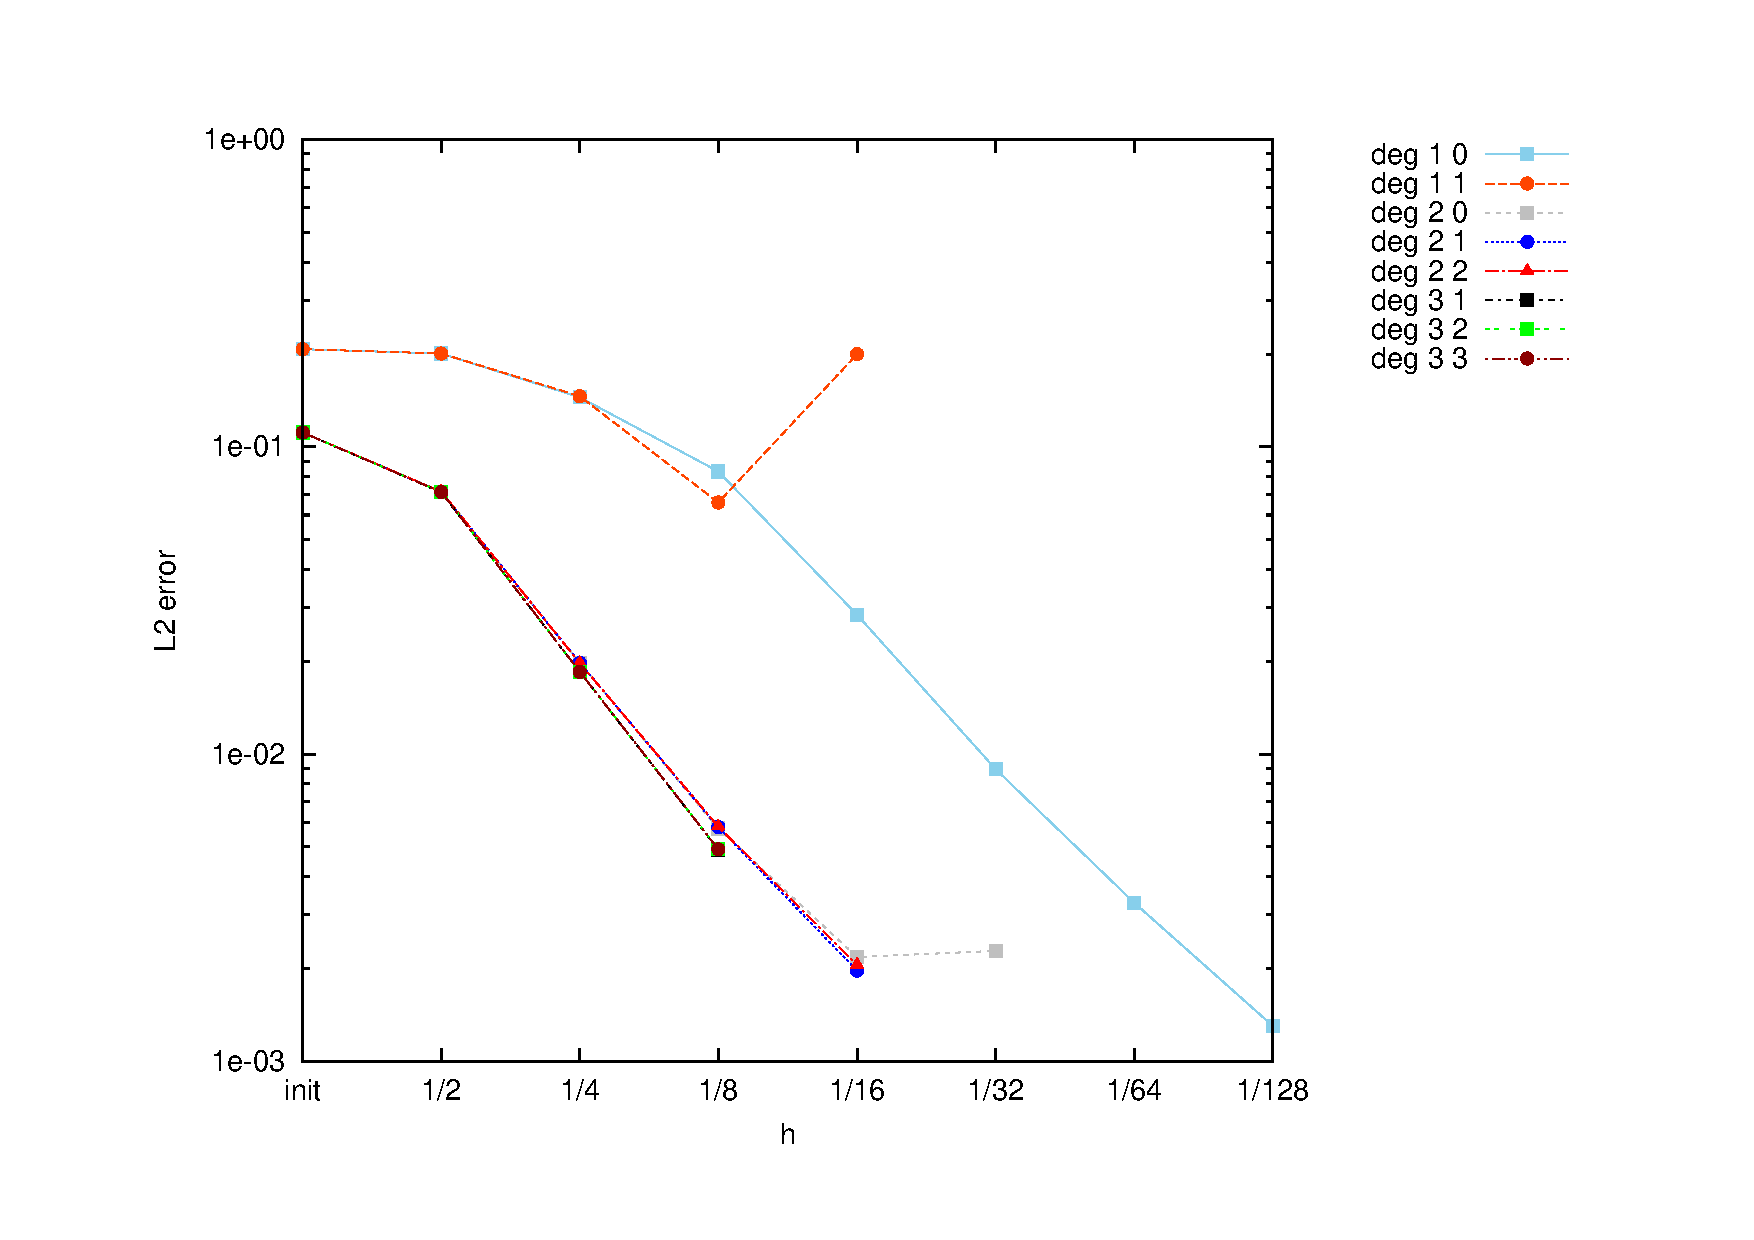
\includegraphics[scale =0.4]{../../FEniCS/diagrams/MA4_Neilan_GradJump_l2.pdf}
	\caption{$L^2$ errors for test case \ref{test dirac} and additional gradient jump penalty}
	\label{fig: l2 errors test 4 jump}
\end{figure}
	
\begin{figure}[H]
		\centering
		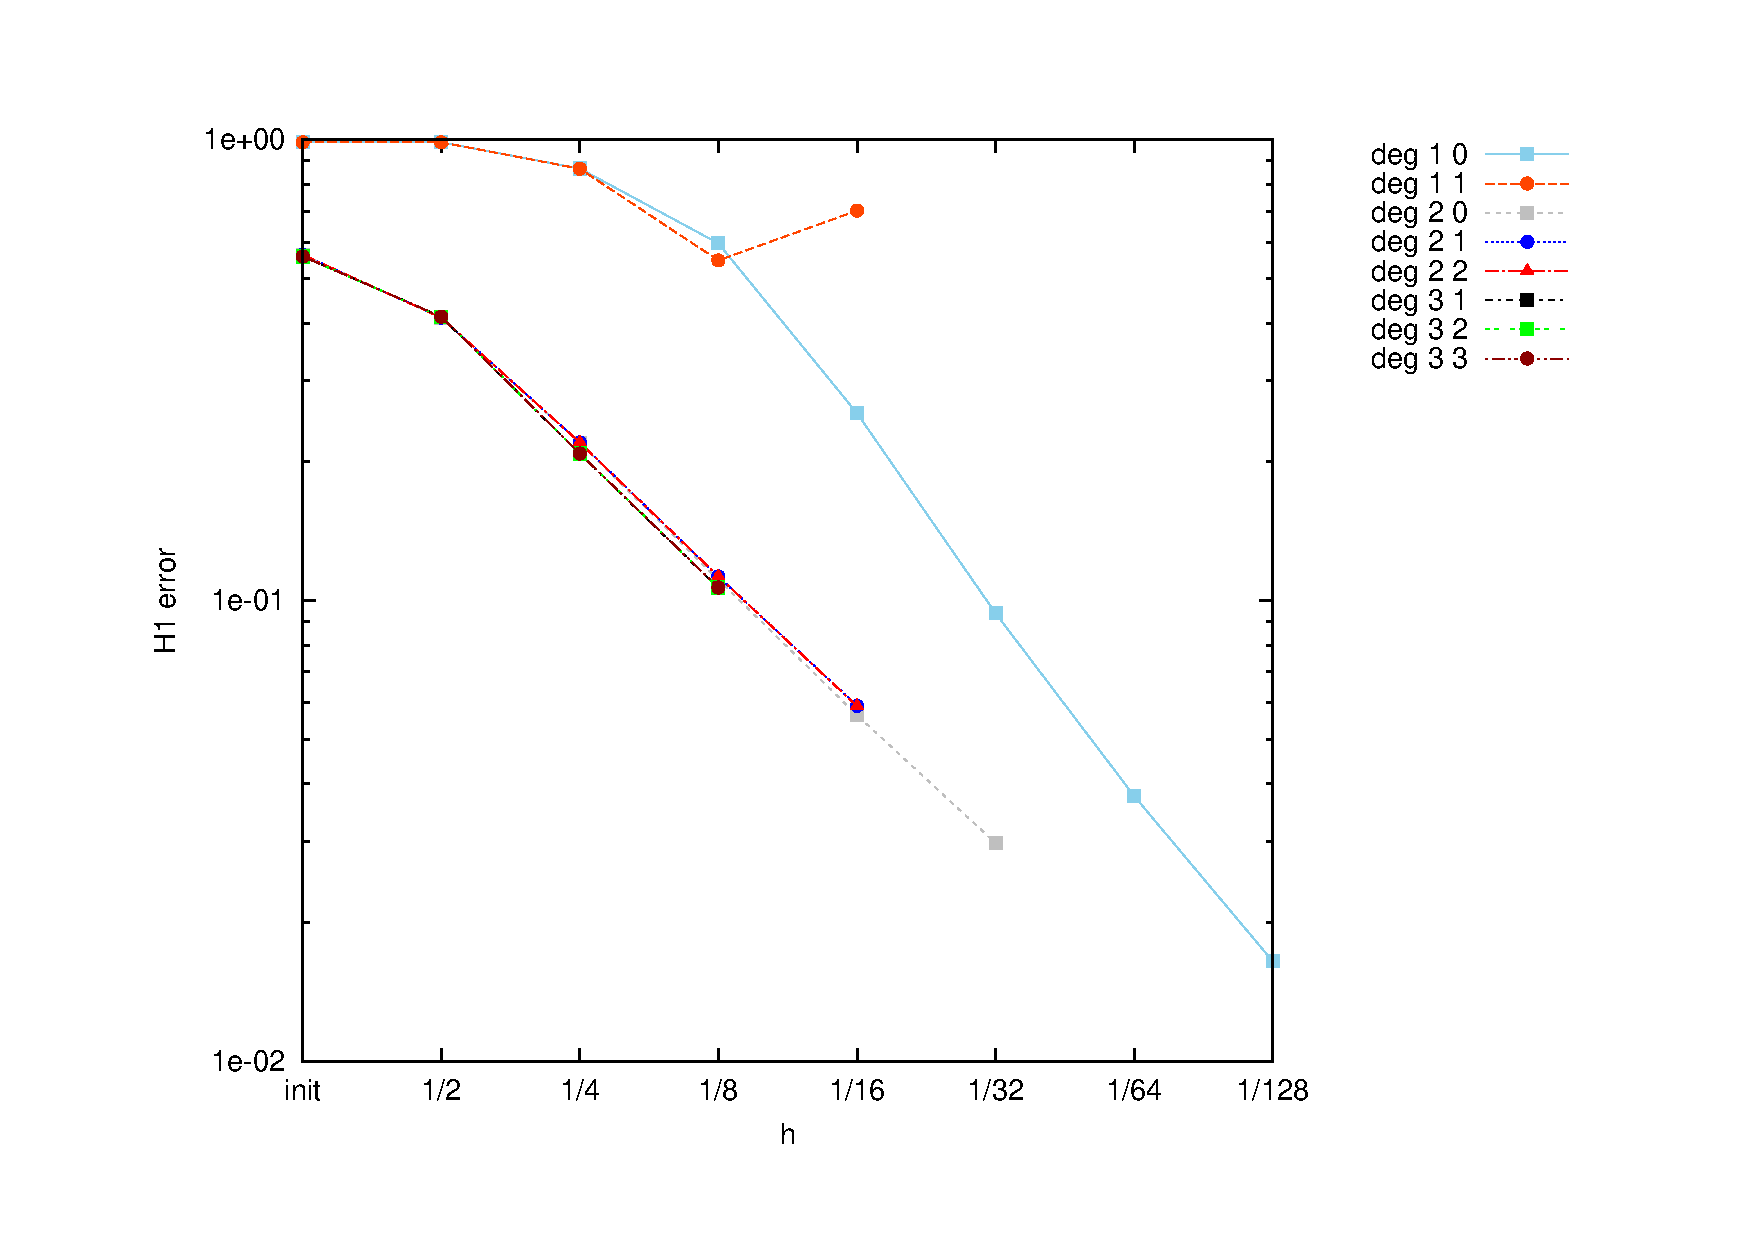
\includegraphics[scale =0.4]{../../FEniCS/diagrams/MA4_Neilan_GradJump_h1.pdf}
	\caption{$H^1$ errors for test case \ref{test dirac} and additional gradient jump penalty}
	\label{fig: h1 errors test 4 jump}
\end{figure}
As before we do not observe much difference between the choices $k=2$ and $k=3$ during the first (converged) refinements. But as the Aleksandrov solution of this test case lacks regularity it is not surprising that increasing the polynomial degree does not effect the error.

It is noticeable that for $k=2$ the $L^2$ error increases after four refinement while the $H^1$ error decreases, we already experienced this behaviour in test \ref{test smooth}.